\subsubsection*{Conventional versus modern neuroscience experimentation}

Conventional system neuroscience experiments heavily constrain the behaviour of
their subjects in order to simplify behavioural and neural analysis.  However,
important aspects of brain function may not be expressed in these constrained
behaviours and these aspects may only manifest in naturalistic experimental
conditions.

% recent foraging experiments
% -> need of advanced machine learning methods to extract information from these experiments

Recent technological advances now allow to build complex naturalistic
experiments, while measuring a large number of experimental variables and
recording from a large number of neurons simultaneously. These advances
allow unrestrained subjects behaviour with precise monitoring of what happens in
the subjects' environment and brain.

Important examples of these experiments are naturalistic foraging experiments,
where freely moving subjects search for food in unrestrained environments.
Foraging studies are currently underway at major research centres around the
world (e.g., the Allen Institute for Brain Research, Janelia Farm, the Max
Plank Institute of Animal Behaviour).

A complication of naturalistic neuroscience experiments is extracting meaning
from the plethora of data that they generate \citep{juavinett22}. Machine
learning methods are specially helpful to address this problem. For example,
they can be used to extract subjects' internal states from behavioural
measurements, to extract low-dimensional latent variables from high-dimensional
neural recordings, and to relate the inferred subjects' internal state to the
neural latent variables.

The data generated by conventional system neuroscience experiments can be
understood by just plotting a few of its variables. However, interpreting the output
of naturalistic experiments is more difficult and machine learning methods
become essential for this.

\subsubsection*{Long-duration and naturalistic experiments at the SWC}
% at the SWC we are performing a new type of foraging experminets

We have developed a new platform that allows housing of mice for several weeks
to months in a large enclosure (\textgreater 2m diameter), while manipulating and
monitoring their behaviour at high spatiotemporal resolution. The arena floor
is tessellated to form a honeycomb of modular hexagonal tiles
(Figure~\ref{fig:arena}a), each of which can be equipped with a newly designed
underground feeder (Figure~\ref{fig:arena}b). Pellets are dispensed onto a
foraging wheel once the mouse has spun it for a pre-defined programmable
distance threshold using its forepaws (fictive digging). By modulating the
digging cost/reward ratio at multiple arena location, this feeder allows the
simulation of different foraging scenarios and probe mice behavioural
strategies. The arena contains up to six scale-equipped nesting modules that
allows housing of mice in the arena and weight monitoring. Mice can live in the
arena for prolonged periods of time weeks to months and express their full
natural behavioural repertoire.

\begin{figure}
    \begin{subfigure}{\textwidth}
        \centering
        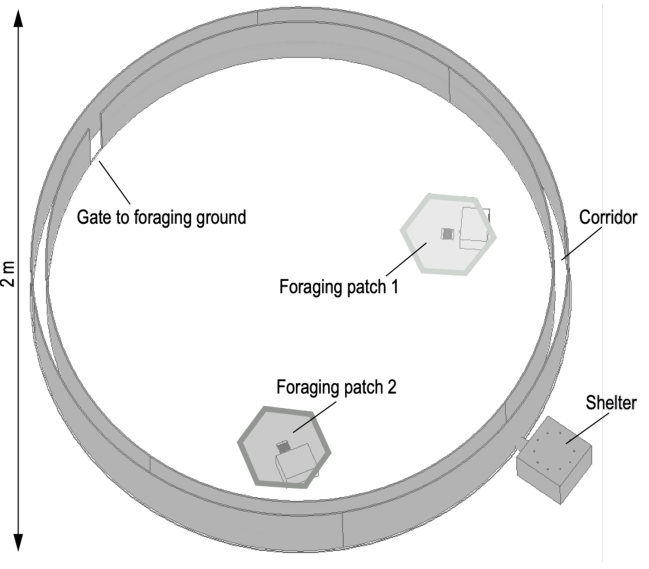
\includegraphics[width=4in]{figures/arena.png}
        \caption{}
    \end{subfigure}
    \par\bigskip
    \begin{subfigure}{\textwidth}
        \centering
        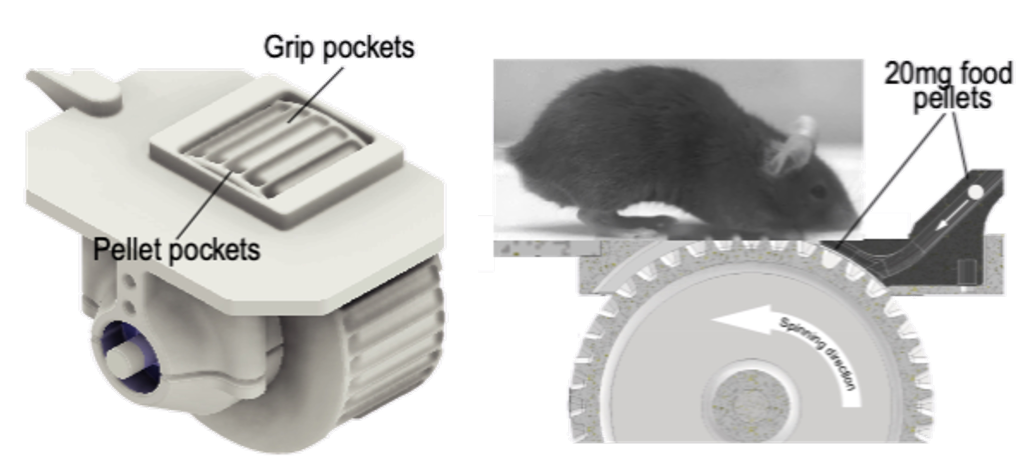
\includegraphics[width=4in]{figures/patch.png}
        \caption{}
    \end{subfigure}
    \caption{Foraging arena (a) and patch (b).}
    \label{fig:arena}
\end{figure}

Behavioural monitoring is achieved by an array of high-speed cameras (up to
15), by which mouse location, mouse identity and body parts can be track in
real time.

Our platforms also enables continuous long term monitoring of neural activity
using Neuropixels probes, the state of the art recording electrode, able to
measure the activity of thousands of neurons simultaneously spanning the entire
brain depth. Using this platform we have collected several week long datasets
both with single mouse and multiple mice. This dataset capture a rich
behavioural repertoire including a foraging behaviour,  social learning task,
defensive and nesting behaviours.

These long-duration experiments are allowing us to address foraging questions
that cannot be studied in shorter experiments. For example, scientifically
these experiments allow us to ask how do mice foraging patterns change across
days, and what are the neural mechanisms underlying these changes.
Statistically, the large amount of data recorded in the new experiments allows
us to estimate parameters of much more complex models than those that can be
fitted to data from conventional system neuroscience experiments.

% normative versus statistical characterization of foraging behavior
% The most common characterization of foraging experiments is a principled one,
% based on the marginal value theorem~\citep{charnov74}. It states that a subject
% will leave a patch when the reward rate of the patch falls below the average
% reward rate in the environment. Naturalistic and long-duration experiments
% allow us to attemp statistical characterizations of foraging experiments

% The naturalistic and long-duration experiments

\subsubsection*{Proposed resource}
% the proposed project

The initial SWC foraging project was supported by core funds from the SWC. The
data it generated has only been analyzed by SWC and Gatsby Unit scientists. %
Due to its uniqueness, we aim to distribute the generated data widely to
benefit the broad scientific community. However the complexity and size of
these data create unprecented challenges for their distribution and analysis. %
Here we propose to mature this foraging project and create a resource to (1)
share data from our foraging experiments to provide scientists across the world
access to unprecedented experimental measurements, (2) share machine learning
software implementations of methods to simulate and analyse these data to
eneable scientists around the world to generated insights from these
recordings, (3) to promote the development of novel tools to simulate and
analyze this data by organising foraging data simulations and analysis
competitions and (4) provide online support to users of the resource to
facilitate their use of the data and methods provided in this resource
(Figure~\ref{fig:resource}).

\begin{figure}
    \begin{center}
        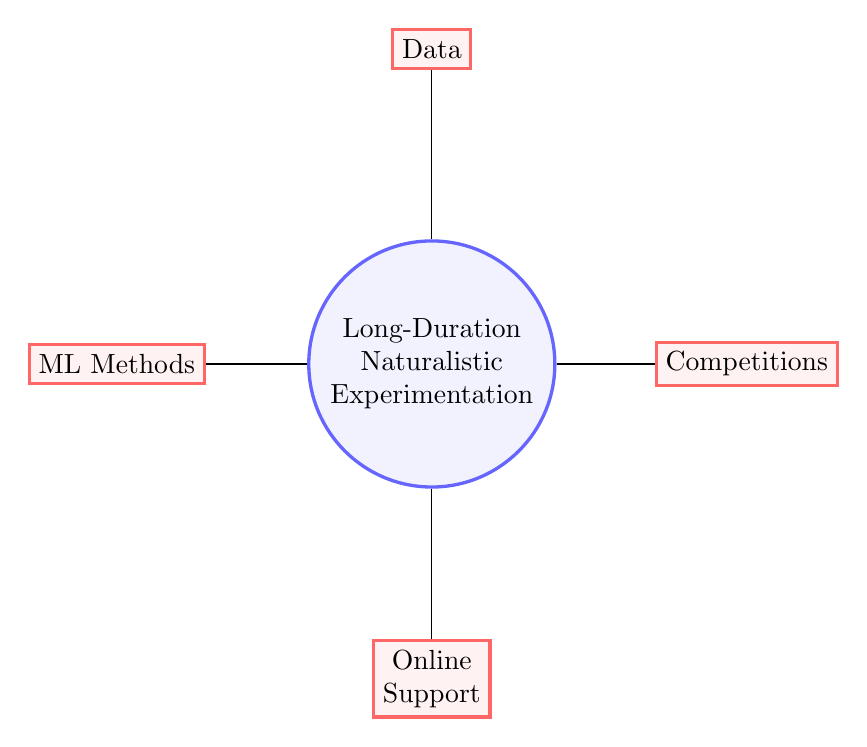
\begin{tikzpicture}[
        node distance=4cm and 1cm,
        centralNode/.style={circle, draw=blue!60, fill=blue!5, very thick,
        minimum size=7mm, align=center},
        itemNode/.style={rectangle, draw=red!60, fill=red!5, very thick,
        minimum size=5mm, align=center},
    ]
    \node[centralNode] (ldnExp)                                 {Long-Duration\\Naturalistic\\Experimentation};
    \node[itemNode]    (dataRepo)           [above of=ldnExp]   {Data};
    \node[itemNode]    (methodsRepo)        [left of=ldnExp]    {ML Methods};
    \node[itemNode]    (competitionsRepo)   [right of=ldnExp]   {Competitions};
    \node[itemNode]    (onlineSupport)      [below of=ldnExp]   {Online\\Support};
    \draw[-] (ldnExp) -- (dataRepo);
    \draw[-] (ldnExp) -- (methodsRepo);
    \draw[-] (ldnExp) -- (competitionsRepo);
    \draw[-] (ldnExp) -- (onlineSupport);
\end{tikzpicture}

    \end{center}
    \caption{Resource theme (blue) and deliverables (red).}
    \label{fig:resource}
\end{figure}

Data generated by our long-duration and naturalistic foraging experiments will
be made publicly available, following FAIR standards, in the
\href{https://dandiarchive.org/}{DANDI} archive.

Whenever possible we will distribute offline and online implementations of all
data analysis methods.
%
Funded by a BBR
award\footnote{\href{https://gow.bbsrc.ukri.org/grants/AwardDetails.aspx?FundingReference=BB\%2FW019132\%2F1}{award details}}
we at the SWC, GCNU and NeuroGEARS are adding machine learning methods to
Bonsai. This project will use will use these methods, add a few more methods to
Bonsai, and use them to intelligently control our long-duration naturalistic
foraging experiments with Bonsai.

We will initially distribute methods that we have already used for our foraging
experiments. For several functionalities we have used more than one method, and
we will distribute all of them. In this way experimental neuroscientists using
our resource should be able to compare different distributed methods and choose
the one more suitable to their needs.

The capability to simulate realistic foraging behaviour is important for our
experiments. First, we often have to decide between several options to
configure our foraging arenas (e.g., should we use two or three foraging
patches? how much distance should mice travel to obtain a pellet? where should
patches be located?). It would be helpful to evaluate the different options on
simulated experiments, rather than evaluating them on expensive real
ones. Second, we are often interested in understanding how much the
behaviour of mice in our experiments differ from optimal behaviour. To address
this issue we will simulate foraging agents and
compare their behaviours with those of real mice.

We will encourage contributions from machine learning method developers
interested in applying their methods to data generated by our foraging
experiments. To motivate them to contribute their methods we will organise data
competitions where participants will be given a data problem to solve (e.g., to
simulate a given environment or to analyse a given dataset), they will provide
their solutions, and we will select the winning one.

\subsubsection*{Intelligent experimental control with Bonsai}

Bonsai is a reactive visual programming environment developed by NeuroGEARS Ltd
that is widely used in Neuroscience for controlling sophisticated neuroscience
experiments. Reactive programs are very different from procedural ones (like C
or Python). The main entity of a reactive program is stream and a reactive
program is a sequence of stream transformations that get an input stream,
transform it, and generate an output one. Reactive programs are ideal to
process online data, like those generated in animal neuroscience experiments.

Not all algorithms that we propose to distribute in this resource admit and
online implementation, however most of them do. Whenever possible, we will
distribute online versions implemented in Bonsai of the methods in this
resource.

Online machine learning methods are relevant to long-duration naturalistic
experimentation for at least two reasons. First the extremely large size of
recorded dataset may forbid storing all raw data and online machine learning
algorithms can help decide what data to store. For instance, we want to record
the behaviour of multiple animals in large arenas with high resolution. This
requires using multiple high-definition cameras to record videos of different
parts of the arena. It is not feasible to store the videos by all cameras in
long duration experiments. To overcome this problem, we can use probabilistic
machine learning methods to track online the positions of the mice in the
arena. When the tracking confidence of this methods is high, we would only save
the high-resolution videos of the cameras filming mice, but when their
confidence is low we would save the videos of all cameras.

Second, we want to make neural interventions informed by online inferences from
machine learning methods. For example, in a foraging experiment we could find
that a neural latent variable peaks before the instant when a mouse start
accelerating to leave the current patch (the latent variable could be estimated
using a Poisson linear dynamical system and the acceleration using a linear
dynamical
system\footnote{\url{https://github.com/joacorapela/lds_python/blob/master/docs/tracking/tracking.pdf}}).
We could hypothesise that the neural population associated with the latent
variable is responsible for the decision of leaving a patch. We could then test
this hypothesis by optogenetically silencing this population while an animal is
on a patch and checking if it leaves the patch or not.

\subsubsection*{Resource background}

In July 2020 the SWC began building hardware and software infrastructure to
record behaviour and neural activity of freely moving mice foraging in large
arenas. Our initial focus was on monitoring behaviour for extended periods of
time. We have been able to record behavioral videos, monitor the movement of
the foraging wheels, register pellet deliveries and record mice weight for up
to two weeks in experiments with two mice.
%
More recently we have been able to record behaviour (as described above) and
neural activity (Neuropixel array, four shanks, 384 electrodes per shank)
continuously for up to 27 hours.
%
Our next target is to record behavioral and electrophysiology data continuously
for one month.

We expect that a position paper describing our foraging experiments will be
published by the end of 2024.

\subsubsection*{Why is the proposed resource unique and timely}

% why is the resource unique and timely

Long-duration and naturalistic experimentation is the future of experimental
neuroscience.  Animal foraging is a central neuroscience problem today and
multiple groups around the world are working on it (e.g., Allen Institute for
Neural Dynamics, Janelia Farm, University of Konstanz). Yet, none of this
groups is focused on the unique long-duration and naturalistic experiments that
we are developing at the SWC.
%
The foraging data and the machine learning methods that we propose to
distribute are key elements for world-class foraging research.
%
If this resource is not created the emergence of naturalistic experimentation
will be delayed and the UK may miss the opportunity of becoming a world leader
on this new type of experimentation.

The US Brain Research through Advancing Innovative Neurotechnologies (BRAIN)
initiative~\citep{jorgensonEtAl15} funded projects focused on data analysis
with advanced machine learning methods for long-duration and complex experiment
that we propose to address in this project. However, no BRAIN initiative
project generated the unique long-duration and naturalistic neuroscience
experimental data that we are creating at the SWC.

We have focused this proposal on applications of naturalistic and long-duration
experimentation to experimental neuroscience. However, this type of
experimentation is relevant to other scientific disciplines. For example, it
could we useful to improve the health of plants. We could perform long-duration
experiments on the wild measuring many quantities from the plant environment
(e.g., water, light, temperature, mineral nutrients, humidity) and from the
plant physiology (e.g., photosynthesis, bud burst). We could then study how the
environment affects plant physiology and health across multiple scales. Close
loop interventions could then be performed (e.g., increasing water delivery) to
improve the plant health.

\subsubsection*{Why are we a suitable team to create this resource?}

We (the SWC, GCNU and NeuroGEARS) are an excellent team to develop the proposed
resource. The SWC is at the forefront of experimental neuroscience research and
has been developing mice foraging experiments for five years. The GCNU is a
leader in computational neuroscience and machine learning, with ample
experience in building methods to characterise neural data, and more recently
in distributing openly machine learning methods. And NeuroGEARS has more than a
decade of experience building high-quality software for experimental
neuroscience. We collaborate extensively in a wide range of projects.

